%! Author = vsharma
%! Date = 25.09.2022
% !TeX spellcheck = en_EN

\chapter{Methodology}

\par AWS enables organizations to dynamically scale their applications and infrastructure.
However, continuously adding new tools and services introduces new security challenges.
According to reports, around 70 percent of organizations IT leaders are concerned about how secure they are in the cloud and 61 percent of small- to medium-sized businesses (SMBs) believe their cloud data is at risk \cite{65}. Although AWS is responsible for securing the infrastructure, it makes it clear to the users to ensure AWS services are properly configured according to best practices to avoid security vulnerabilities.

\par This research emphasizes identifying the efficiency of the open-source security assessment tool, Prowler.
To do so, different approaches are identified. This chapter explains the used approaches.


\section{Identification of Security vulnerabilities and Exploits}

\par AWS provides more than 100 services, and each of these services is vulnerable to security attacks.
These security vulnerabilities can be classified corresponding to each of the AWS services.
This research work is limited to 5 AWS services namely IAM, EC2, S3, RDS, and Lambda.
Columns 1 and 2 in table \ref{tab:classificationofsecurityvulnerabilities} lists the different security
vulnerabilities based on literatures, OWASP vulnerability list \cite{43}, CISA \cite{42}, IDC \cite{41}.

\begin{longtable}{|p{10cm}|p{2.4cm}|p{2cm}|}
    \hline
    \textbf{Security Vulnerabilities} & \textbf{Service} & \textbf{Prowler Check}\\
    \hline
    Avoid the use of the root account & IAM & Check11 \\
    \hline
    MFA is enabled for all IAM users & IAM & Check12 \\
    \hline
    Credentials unused for 90 days or greater are disabled & IAM & Check13 \\
    \hline
    Access keys are rotated every 90 days or less & IAM & Check14 \\
    \hline
    IAM password policy requires at least one uppercase letter & IAM & Check15 \\
    \hline
    IAM password policy requires at least one lowercase letter & IAM & Check16 \\
    \hline
    IAM password policy requires at least one symbol & IAM & Check17\\
    \hline
    IAM password policy requires at least one number & IAM & Check18\\
    \hline
    IAM password policy requires a minimum length of 14 or greater & IAM & Check19\\
    \hline
    IAM password policy prevents password reuse & IAM & Check110\\
    \hline
    IAM password policy expires passwords within 90 days or less & IAM & Check111\\
    \hline
    Password expiration requires an administrator reset & IAM & \\
    \hline
    Allow users to change their own password & IAM& \\
    \hline
    Insider Threat & IAM & Extra774\\
    \hline
    Access key for the root account & IAM & Check112 \\
    \hline
    Instances created from Malicious AMI & EC2 & Check76\\
    \hline
    User data public exposure & EC2 & Extra741\\
    \hline
    Server-Side Request Forgery & EC2 & Extra786\\
    \hline
    Denial of Wallet & EC2, Lambda &\\
    \hline
    Public exposure of S3 buckets & S3 & Check73\\
    \hline
    Unencrypted S3 buckets & S3 & Extra764\\
    \hline
    GhostWriter & S3 & Extra771 \\
    \hline
    Publicly accessible RDS instances & RDS & Check78\\
    \hline
    Unencrypted RDS Instance & RDS & Extra735\\
    \hline
    Resources running in an AWS classic resource & RDS & \\
    \hline
    Default data retention & RDS & Extra739\\
    \hline
    Lambda functions have a public resource-based policy & Lambda & Extra798 \\
    \hline
    Publicly accessible AWS account & Lambda & Extra7145 \\
    \hline
    Public lambda function URL & Lambda & Extra7179 \\
    \hline
    Public lambda function URL Cors & Lambda & Extra7180 \\
    \hline
    Insecure Management of Secrets & Lambda & Extra760\\
    \hline
    Poisoning the Well & Lambda & \\
    \hline
    \caption{Prowler Checks and their mapping for Security Vulnerabilities}
    \label{tab:classificationofsecurityvulnerabilities}
\end{longtable}

\section{Prowlers Validation}

\par Prowler scans the AWS account to check for overly permissive IAM permissions, potential vulnerabilities, and best practice violations. Prowler runs 49 checks against the Center for Internet Security (CIS) AWS Foundations Benchmark and over 40 checks related to HIPAA and GDPR compliance. Prowler constantly checks the AWS accounts against the CIS benchmarks for the AWS Cloud. Thus, ensuring that the organization is operating in accordance with guidelines developed by industry consultants, audit and compliance organizations, software developers, operations specialists, security research organizations, government agencies, and legal experts \cite{66}.

\par To determine the efficiency of Prowler against security vulnerabilities two approaches are identified.
The first approach is a test-driven approach, it’s a manual approach and the second approach uses an open-source application to evaluate the efficiency of Prowler against the identified security vulnerabilities \cite{37}.

\par In the end, another open-source assessment tool called ScoutSuite is used to perform the security assessment of the AWS account.
After the assessment using ScoutSuite finishes, the results are recorded.
The comparison between the assessment performed by the two open-source security
assessment tools are shown in the next chapter.

\subsection{Using Test Driven Approach}

\par A test case is a set of actions performed on a system to determine if it functions correctly. Test cases helps
in determining if different features within a system are performing as expected and to confirm that the system
satisfies all related standards, customer requirements and guidelines \cite{86}. This manual approach determines the
efficiency of Prowler against the identified security vulnerabilities listed in table \ref{tab:classificationofsecurityvulnerabilities}.

\par Prowler provides several checks to perform security assessments. These checks help determine whether good practices are being followed to secure the set of resources. For each security assessment check in Prowler, we develop test cases to verify the positive and negative scenarios. In the end, the efficiency of Prowler is determined against the identified security vulnerabilities.

\subsubsection{Algorithm and Flowchart}

\begin{figure}
    \centering
    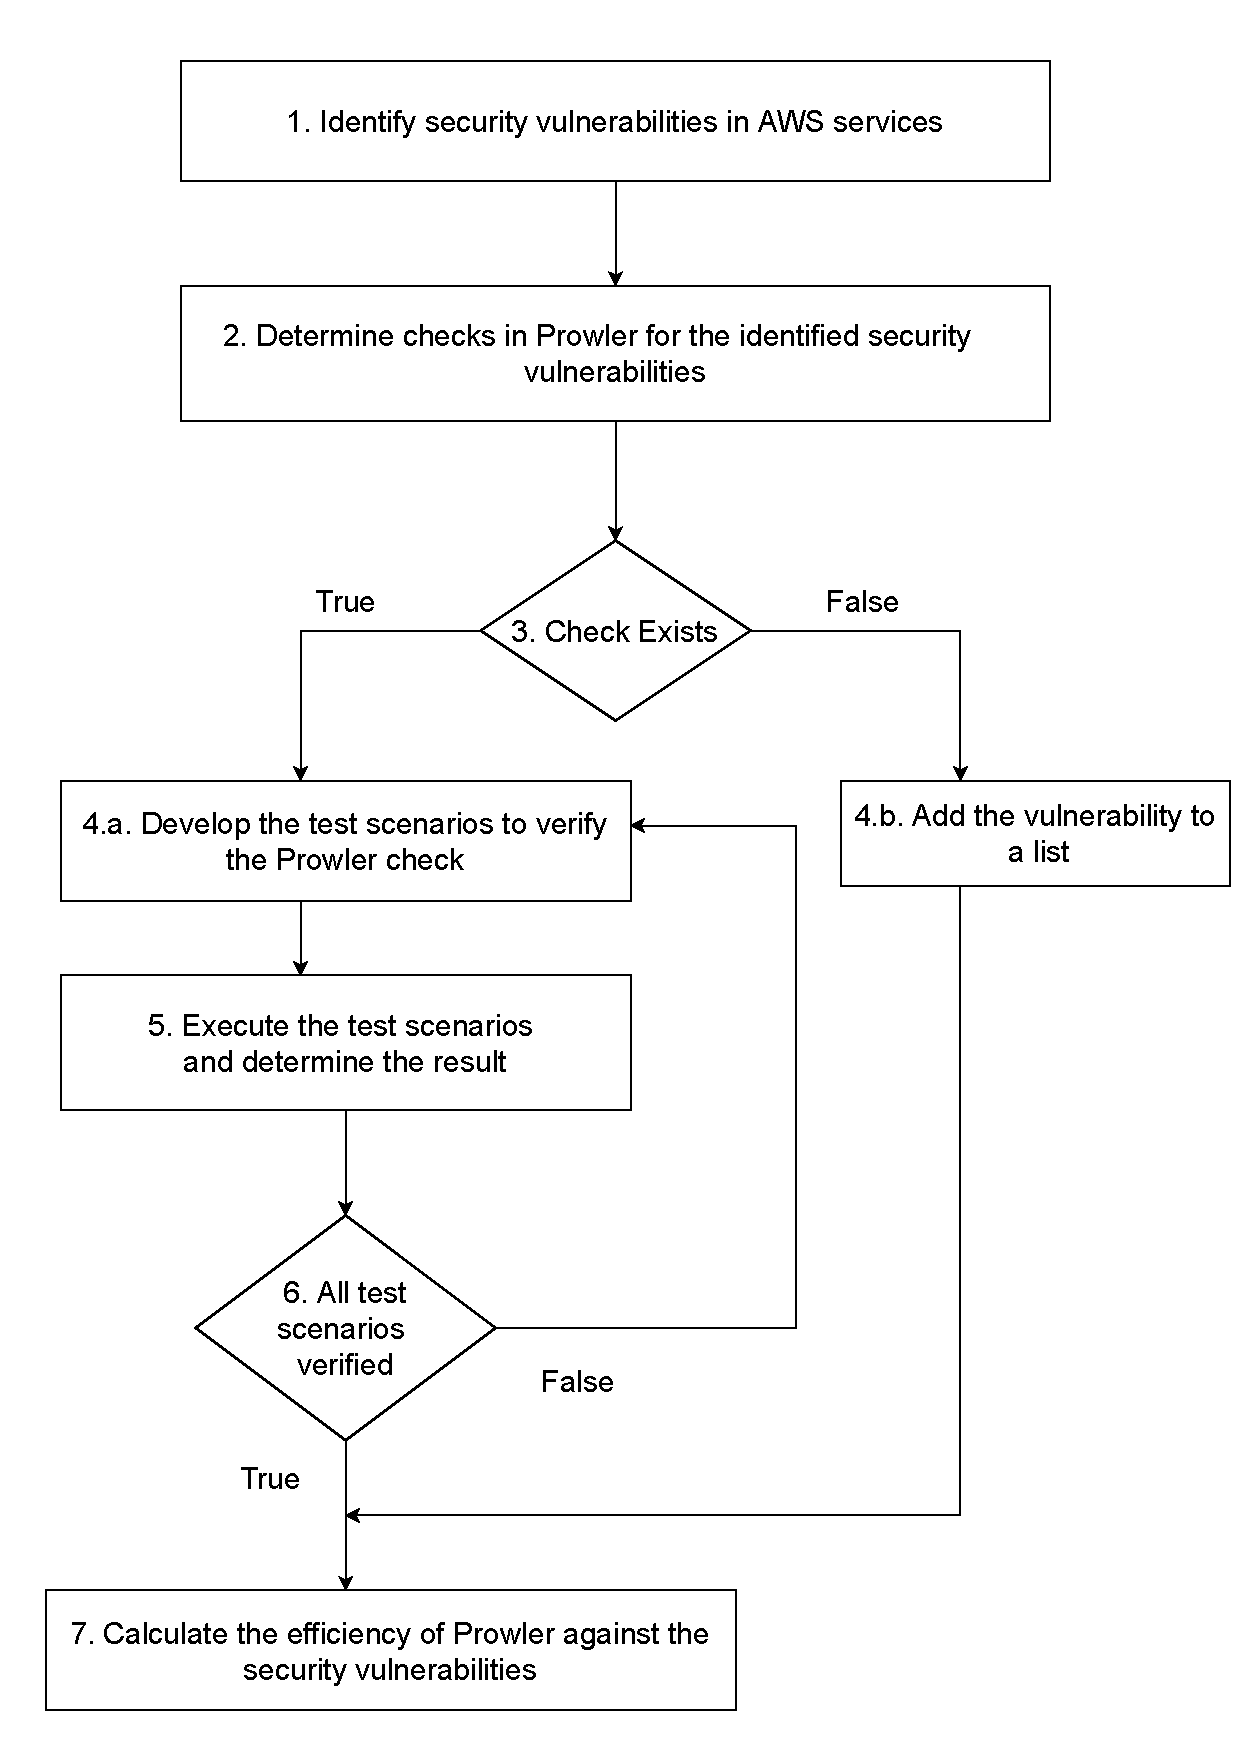
\includegraphics[width=\textwidth]{flowdiagram.pdf}
    \caption{Security vulnerability Assessment flow diagram}
    \label{fig:flowdiagram}
\end{figure}
\begin{itemize}
    \item As an initial step, the process starts by identifying the security vulnerabilities in the five AWS services.
    The different security vulnerabilities are identified based on literatures, OWASP vulnerability list \cite{43}, CISA \cite{42}, IDC \cite{41}.
    This is highlighted as Step 1 in the flow diagram \ref{fig:flowdiagram}.
\end{itemize}
\begin{itemize}
    \item After the identification of security vulnerabilities, the next step is to identify checks in Prowler that assesses the security vulnerabilities identified in step 1.
    This corresponds to steps 2 and 3 in the flow diagram \ref{fig:flowdiagram}.
\end{itemize}
\begin{itemize}
    \item For each check in Prowler develop the test scenarios in python and verify the test scenarios. The result of the test scenarios is noted. These are steps 4.a and 5 in the flow diagram. This process repeats until all the possible checks are verified successfully.
\end{itemize}
\begin{itemize}
    \item If a check does not exist in Prowler for the security vulnerability, add the security vulnerability in a separate list.
    Step 4.b in the flow diagram \ref{fig:flowdiagram} highlighted this process.
\end{itemize}
\begin{itemize}
    \item In the end, the efficiency of Prowler is calculated between the verified security vulnerabilities using the checks in Prowler and the security vulnerabilities identified initially in Step 1 of the flow diagram.
    This is represented as Step 7 in the flow diagram \ref{fig:flowdiagram}.
\end{itemize}


\par The test cases are developed for each check in Prowler.
As we see from the listing
4.1, the method check15\_require\_upper\_case\_characters() calls the test case methods
for positive and negative scenarios.
The positive scenario is verified using the method
check15\_require\_upper\_case\_characters\_true() and the negative test scenario is verified
using check15\_require\_upper\_case\_characters\_false().

\par Python boto3 \cite{67} library is used in the test cases.
Boto3 is the Python SDK for AWS
that allows creating, updating, and deleting AWS resources directly from your Python
scripts.

\par As a first step, for each scenario the AWS resource such as IAM, EC2, etc. are enabled using boto3 \cite{67}. Upon enabling the resource, the method associated with the resource is determined and used to set the value on the argument, for example, RequireUppercaseCharacters is set to True in this case. After setting the required value on the argument, the check is executed. After the execution of the check finishes, the return code for the test scenario is determined. Once the return code is obtained, it is verified. Only after the verification is successful, the security vulnerability is added to the list of security vulnerabilities verified using prowler.


\lstset{frame=lines}
\lstset{caption={Test code implementation for Prowler assessment}}
\lstset{label={lst:code_check15}}
\lstset{basicstyle=\footnotesize\ttfamily}
\lstset{numberstyle=\tiny\color{cyan}}
\lstset{keywordstyle=\color{red}}
\lstset{identifierstyle=\color{blue}}
\lstset{stringstyle=\color{orange}}
\lstset{commentstyle=\itshape\color{purple!40!black}}
\lstset{
    numbers=left,
    firstnumber=1,
    numberfirstline=true,
    numberstyle=\tiny\color{green},
}

\begin{lstlisting}[language=Python]
	def check15_require_upper_case_characters_true(self):
            client = boto3.client('iam')
            client.update_account_password_policy(RequireUppercaseCharacters=True)
            response = subprocess.run(["./prowler", "-c", "check15"])
            return response.returncode
        def check15_require_upper_case_characters_false(self):
            client = boto3.client('iam')
            client.update_account_password_policy(RequireUppercaseCharacters=False)
            response = subprocess.run(["./prowler", "-c", "check15"])
            return response.returncode
        def check15_require_upper_case_characters(self):
	    uppercasetrue = self.check15_require_upper_case_characters_true()
	    uppercasefalse = self.check15_require_upper_case_characters_false()
	    if uppercasetrue == 0 and uppercasefalse == 3:
	        self.determine_prowler_matrix('RequireUppercaseCharacters')
\end{lstlisting}


\par Similar steps are followed for verifying all the possible scenarios for different Prowler checks. At the end, when all the checks in Prowler are verified, the efficiency of Prowler is calculated.

\subsection{Using Open-Source Application}

\par The term open source refers to something that can be modified and shared among people because its design is publicly accessible.
The open-source software application is an application that is distributed with its source code, making it available
for use, modification, enhancement, and distribution with its original rights \cite{68}.

\par \par In this approach, an open-source web application developed in Angular.js, and Java Spring boot are used \cite{69}.
Every organization whether government or private uses an information system to store data of their staff.
The employee management system is intended to organize Human Resources (HR) and other departments' work processes.
It is an application-based system that is used by employers to monitor and manage employees from different work locations.
The employee management system provides features that include the ability to add, update, and delete employee information.
The application interface also provides a feature to list all the employees within the organization.
When a new employee joins the company, the information is added to the database.
In case of a mistake in the employee information, the application enables the feature to make corrections to the employee information.
In case an employee leaves the organization, the employee information can be deleted from the application database.

\subsubsection{Infrastructure architecture}

\begin{figure}
    \centering
    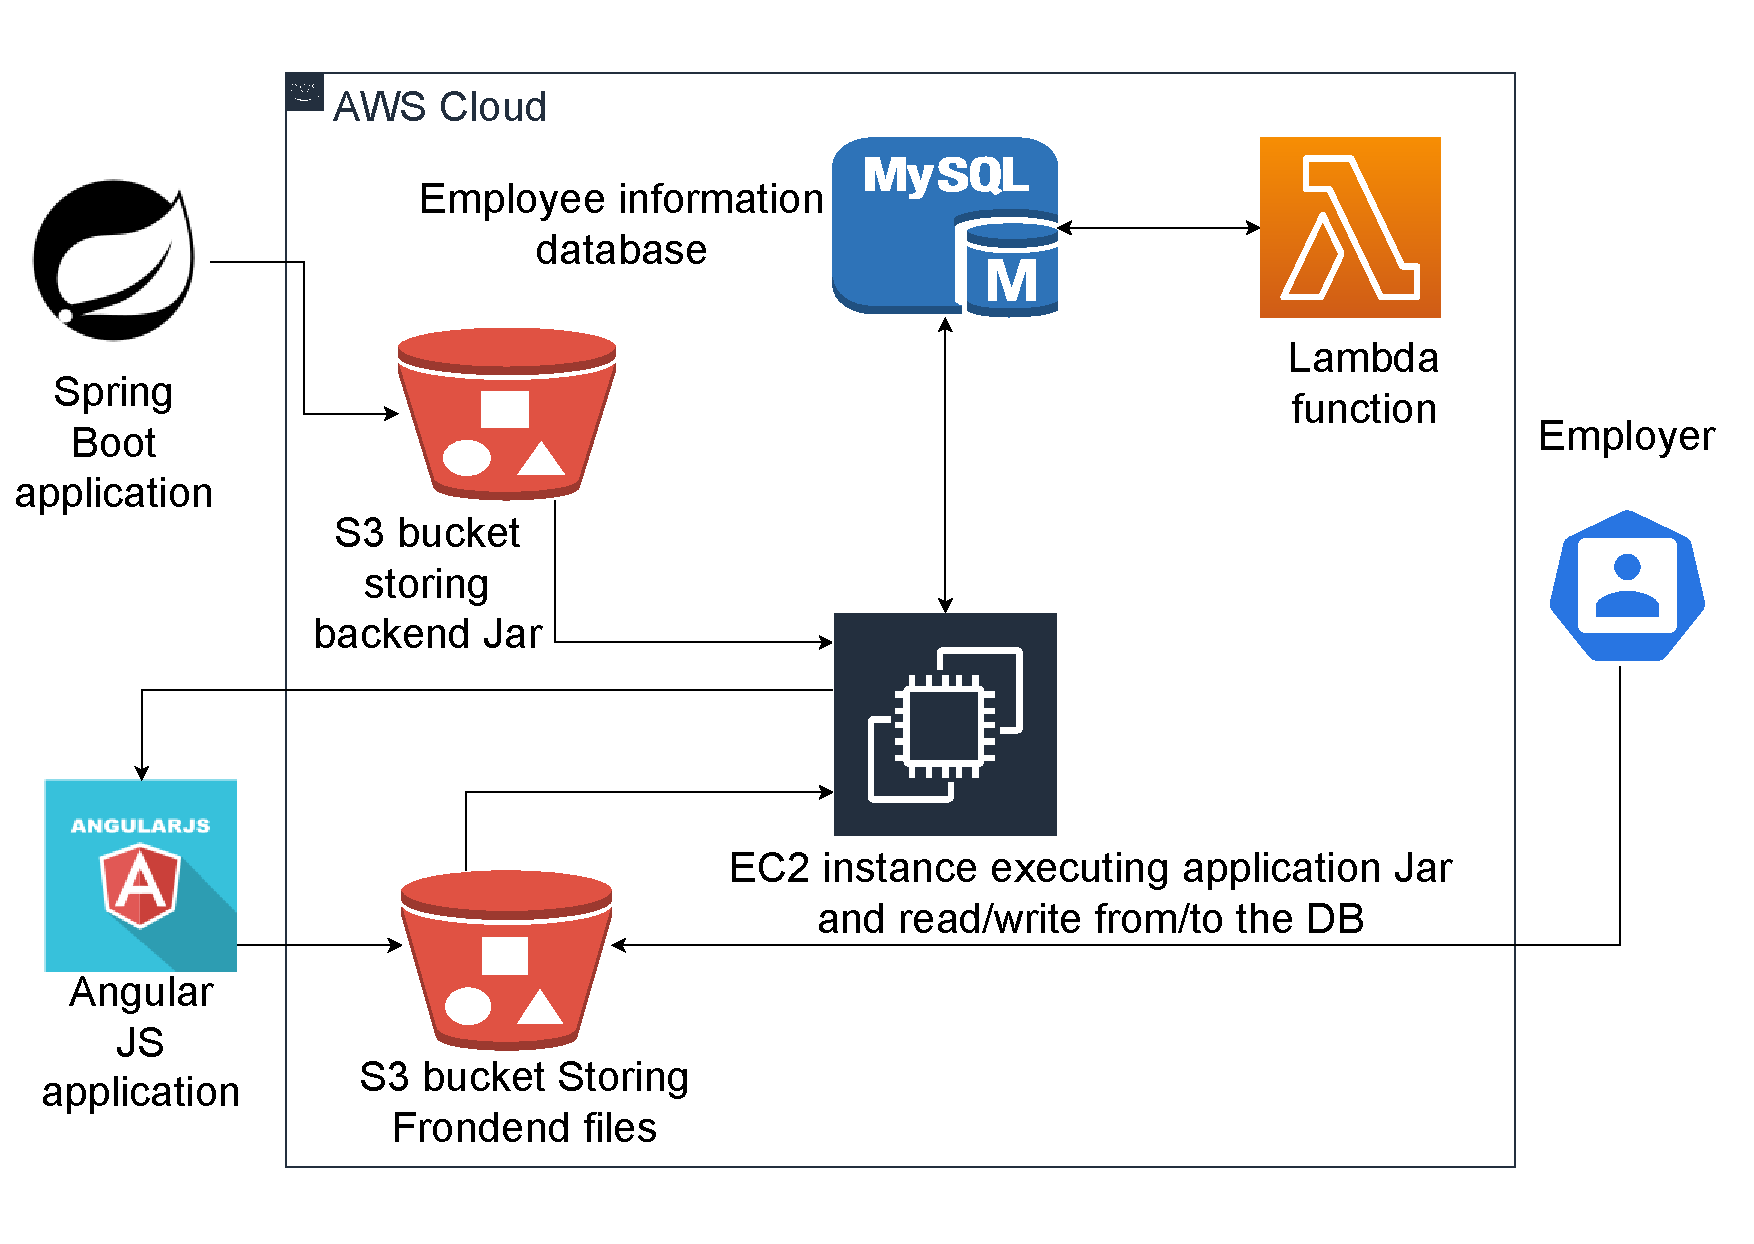
\includegraphics[width=\textwidth]{infrastructure_architecture.pdf}
    \caption{Infrastructure architecture}
    \label{fig:infrastructure_architecture}
\end{figure}

\par The architectural view of the open source application infrastructure is shown in the figure
\ref{fig:infrastructure_architecture}.
The application employs AWS services namely IAM, RDS, S3, EC2, and Lambda.
Below is a detailed explanation that helps to understand the role of each AWS service.

\par IAM

\par The application requires the creation of buckets, databases, ec2 instances, and lambda function and carries out the
execution of commands to perform security assessment using Prowler and ScoutSuite \cite{70}.

\par To perform these operations, the user needs to be assigned the required permissions.
Based on the leave privilege principle the user should only be assigned the permission needed to perform the task.
If a user does not need an access right, then the user must should not be assigned such access right \cite{81}.
AWS IAM service assigns the required permission to the user.
To create and write to the s3 bucket, the user is assigned \textit{s3:CreateBucket} and \textit{s3:PutObject} permission \cite{82}.
To launch the ec2 instance, \textit{ec2:RunInstances} permission is added to the user \cite{83}.
To create the database, \textit{rds:CreateDBCluster} permission is assigned to the user \cite{85}.
To create and execute the lambda function, \textit{lambda:CreateFunction} is added to the user \cite{85}.
\hfill \break
\par S3

\par The application backend of the employee management application as described above is developed in Spring boot and the frontend is developed in Angular.JS. The developed application is available in version control systems such as GitHub, Bitbucket, etc.
With the help of CI/CD, the application code is deployed in the AWS cloud.
CI/CD combines the practices of continuous integration and continuous delivery.
It automates the manual human intervention traditionally needed to get new code from a commit into production such as build, test, and deploy, as well as infrastructure provisioning.
It helps the developers to make changes to code that are then automatically tested and pushed out for delivery and deployment \cite{71}.

\par The required application package, Jar in case of spring boot application, and modules in case of angular.js application are stored in S3 buckets.
For the application to be accessed by the HR\/employer, static web hosting is enabled for the bucket containing angular.js application files.


\hfill \break

\par RDS

\par Amazon RDS help to set up, run and scale database services in the cloud.
The employee management application enables adding, updating, and deleting the employee’s information.
This employee information is stored in the database.
The database details are added to the backend spring boot application which connects to the database to perform the required database operation in response to the request from the frontend angular application by making an API call.

\hfill \break
\par EC2

\par The S3 bucket stores the Java spring boot application jar.
The Jar contains the code implemented to perform different application operations.
For the web application to function, the backend application needs to be run.
To do so an EC2 instance is created.
The backend spring boot application jar is downloaded from the S3 bucket to the ec2 instance.
Once the Jar is downloaded, it is run on the EC2 instance using the command \textit{java -jar applicationname.jar}.

\hfill \break
\par Lambda

\par Lambda services execute code without provisioning servers.
The application infrastructure contains a lambda function that makes an API call to the RDS database.
The function retrieves the information of employees within the organization.
The database details are hardcoded as a connection string within the lambda function.
Upon successful validation of the database details, the request is made to fetch the employee’s information.
\begin{figure}
    \centering
    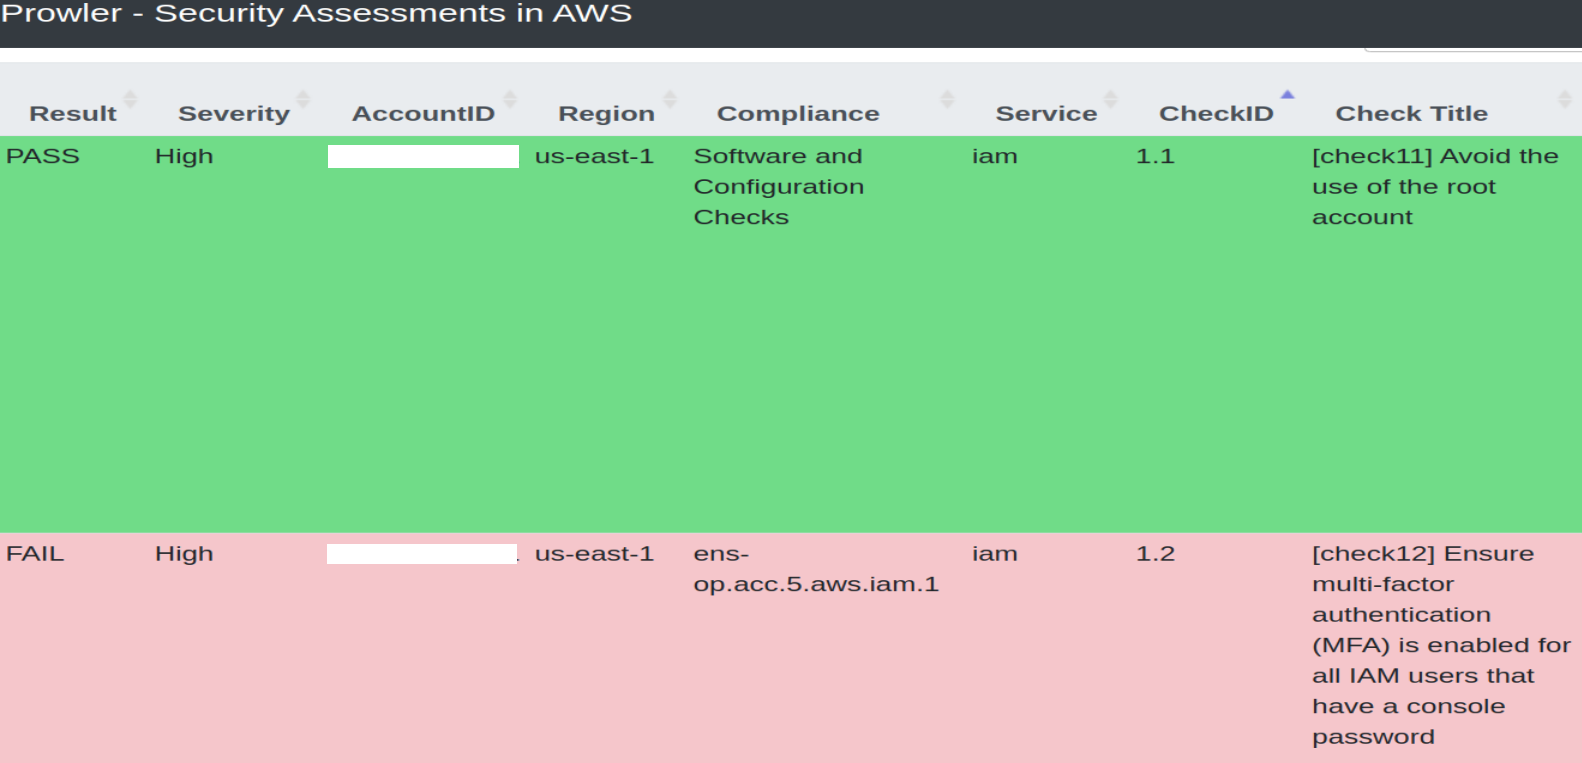
\includegraphics[width=175mm,height=12cm]{prowlerAssessment.PNG}
    \caption{Prowler security assessment}
    \label{fig:prowlerassessmentreport}
\end{figure}
\par To ensure the safety of the infrastructure, a security assessment needs to be performed to identify any security vulnerabilities that might have been introduced while setting up the infrastructure. This is performed by making use of security assessment tools such as Prowler. The assessment starts by executing the command \textit{./prowler}. Once the assessment completes, the assessment report is generated. This report provides details about the security vulnerabilities associated with different AWS services within the infrastructure.

Figure \ref{fig:prowlerassessmentreport} shows the snippet of the assessment report generated using Prowler.


\hfill \break
\section{ScoutSuite}

\par Scout Suite is an open source multi-cloud security-auditing tool.
It is used by external and internal security analysts to assess cloud environments.
Scout Suite  uses the API exposed by the cloud service provider to collect configuration data from high security risk areas for manual audit by researchers.
Based on configuration gathered data, it shows security risks and issues present in the infrastructure \cite{72}.
\hfill \break
\par Features of ScoutSuite
\begin{itemize}
    \item Persistent monitoring: ScoutSuite is a user-friendly tool that provides the ability to constantly monitor
    the public cloud accounts.
    Persistent monitoring helps to review computing resources for workflow optimization while ensuring ceaseless service availability and high performance.
    It ensures tracking of the issues as they occur.
    It also aids in the evaluation of resource availability, program speed, and resource levels, to further help predict vulnerability attacks before their occurrence \cite{73}.
\end{itemize}
\begin{itemize}
    \item Agnostic platform: Agnostic Platform refers to tools or applications that are compatible with any cloud
    infrastructure and can be moved without any operational issues to and from different cloud environments.
    An agnostic platform can be compared favorably to cloud-native tools that tend to be platform-specific and that can create visibility issues for businesses operating in a multi-cloud or hybrid cloud environment.
    Using cloud-agnostic tools such as ScoutSuite benefits from greater visibility across their cloud environment and gives them more clarity about how their ecosystem works, leading to better-informed decision making \cite{73}.
\end{itemize}


\hfill \break

\subsection{Deploying ScoutSuite}

\par Scout Suite is a multi-cloud tool namely Google Cloud Platform, AWS, Microsoft Azure, Alibaba Cloud (alpha), and
Oracle Cloud Infrastructure (alpha). In this research work, ScoutSuite is deployed on an AWS EC2 instance with an
IAM role configured \cite{73}.

\par Once the EC2 instance is running, the instance is connected.
Connection to the EC2 instance is established using EC2 Instance Connect, Session Manager, SSH client example Putty, and EC2 serial console.
After the EC2 instance is connected, it must be configured.
Configuring the EC2 instance is done using the command \textit{aws configure}.
During configuration, it prompts for "Access key ID," "Secret Access Key," "Default Zone," and "Output format".
Once configured, the virtual environment must be installed.
Installation of the virtual environment is done by using the command \textit{pip3 install virtualenv}.
After installing virtualenv, a virtual environment must be created, to do this the command \textit{virtualenv -p python3 venv} is executed.
The next step is to install ScoutSuite on the virtual environment.
Installing virtual environment requires running the commands \textit{source venv/bin/activate} and \textit{pip3 install scoutsuite}.
The final step is to test and run ScoutSuite. Verification of the installation is done by running the command \textit{scout --help}.
The tool's usage syntax for different cloud environments is shown using the help command.
ScoutSuite is run by executing the command\textit{scout aws}.
Once the command execution finishes, the HTML report gets
generated in the current working directory \cite{72}.

Figure \ref{fig:deployscoutsuite} shows the snippet of the report generated using ScoutSuite.

\begin{figure}
    \centering
    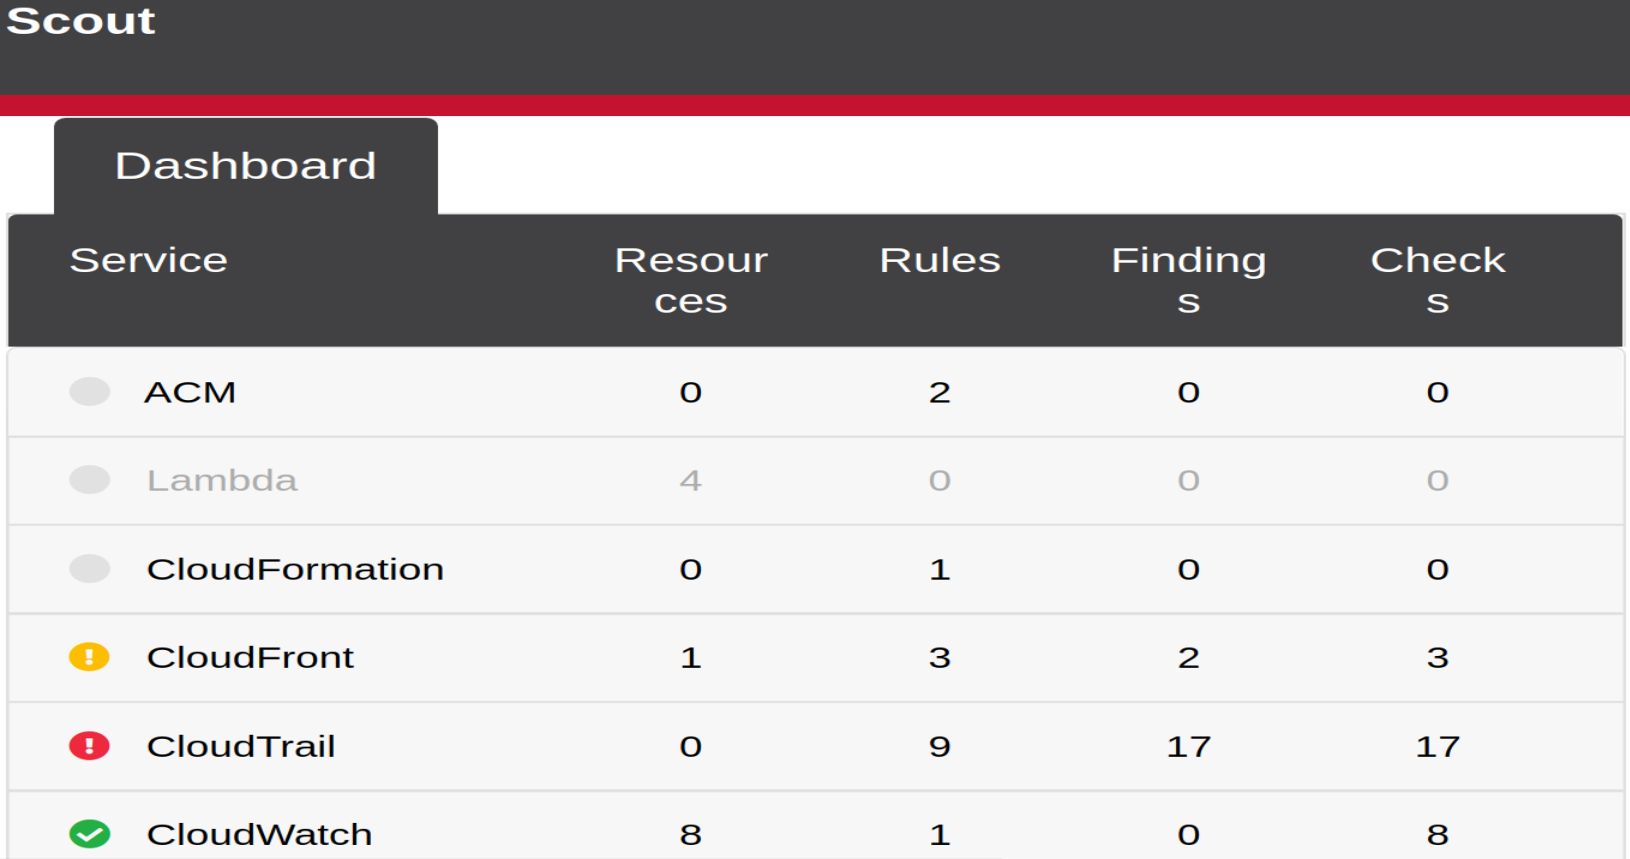
\includegraphics[width=\textwidth]{scoutAssessment.PNG}
    \caption{ScoutSuite Report}
    \label{fig:deployscoutsuite}
\end{figure}